\subsection{Missing Data}
Upon inspection of the provided \textit{match\_history.csv} file, it became clear that numerous data points are missing. Throughout the dataset, for at least one country each, there is data missing from the \textit{offense\_score, midfield\_score, defense\_score} and \textit{goalkeeper\_score} fields. When reading the data, these missing values are interpreted as `NaN' - a value that cannot be used in any regression technique. Since the quality of a model's output is directly correlated to its input, as mentioned above, we tried numerous methods of handling the fact that these values are missing; in order to be able to train regression models properly with a complete dataset.

\subsection{Types of Missing Data}
\label{sec:miss data}
As previously stated, the efficacy of a model and the quality of the dataset are directly correlated - insufficient or poor quality data produces inaccurate and meaningless predictions. 

In any dataset, missing data can be categorised into four distinct types \cite{missing_data}: 
\begin{enumerate}
    \item Missing completely at random
    \item Missing at random
    \item Missing depending on unobserved predictors
    \item Missing depending on the missing value itself
\end{enumerate}
In our case, the missing data can be classified as the second of these types - with the missing data occurring at random rates throughout the dataset - some countries have more missing data values than others. In particular, there are seventeen countries that are missing an entire feature. For example, Zambia has no \textit{goalkeeper\_score} or \textit{defense\_score} throughout the entire dataset; this adds a further layer of complexity.

\subsection{Replacing With Constant}
Our initial approach was simply to find all `NaN' values after the dataset had been read and replace them with a zero. This is extremely fast to execute, however, leads to poor model performance since in most cases, zero is an extremely inaccurate value to replace missing values - with almost all score features being valued above 50. This is very evident when graphing the four aforementioned features - no country has a value for any of the aforementioned features that are remotely close to zero.

\begin{figure}[H]
    \centering
    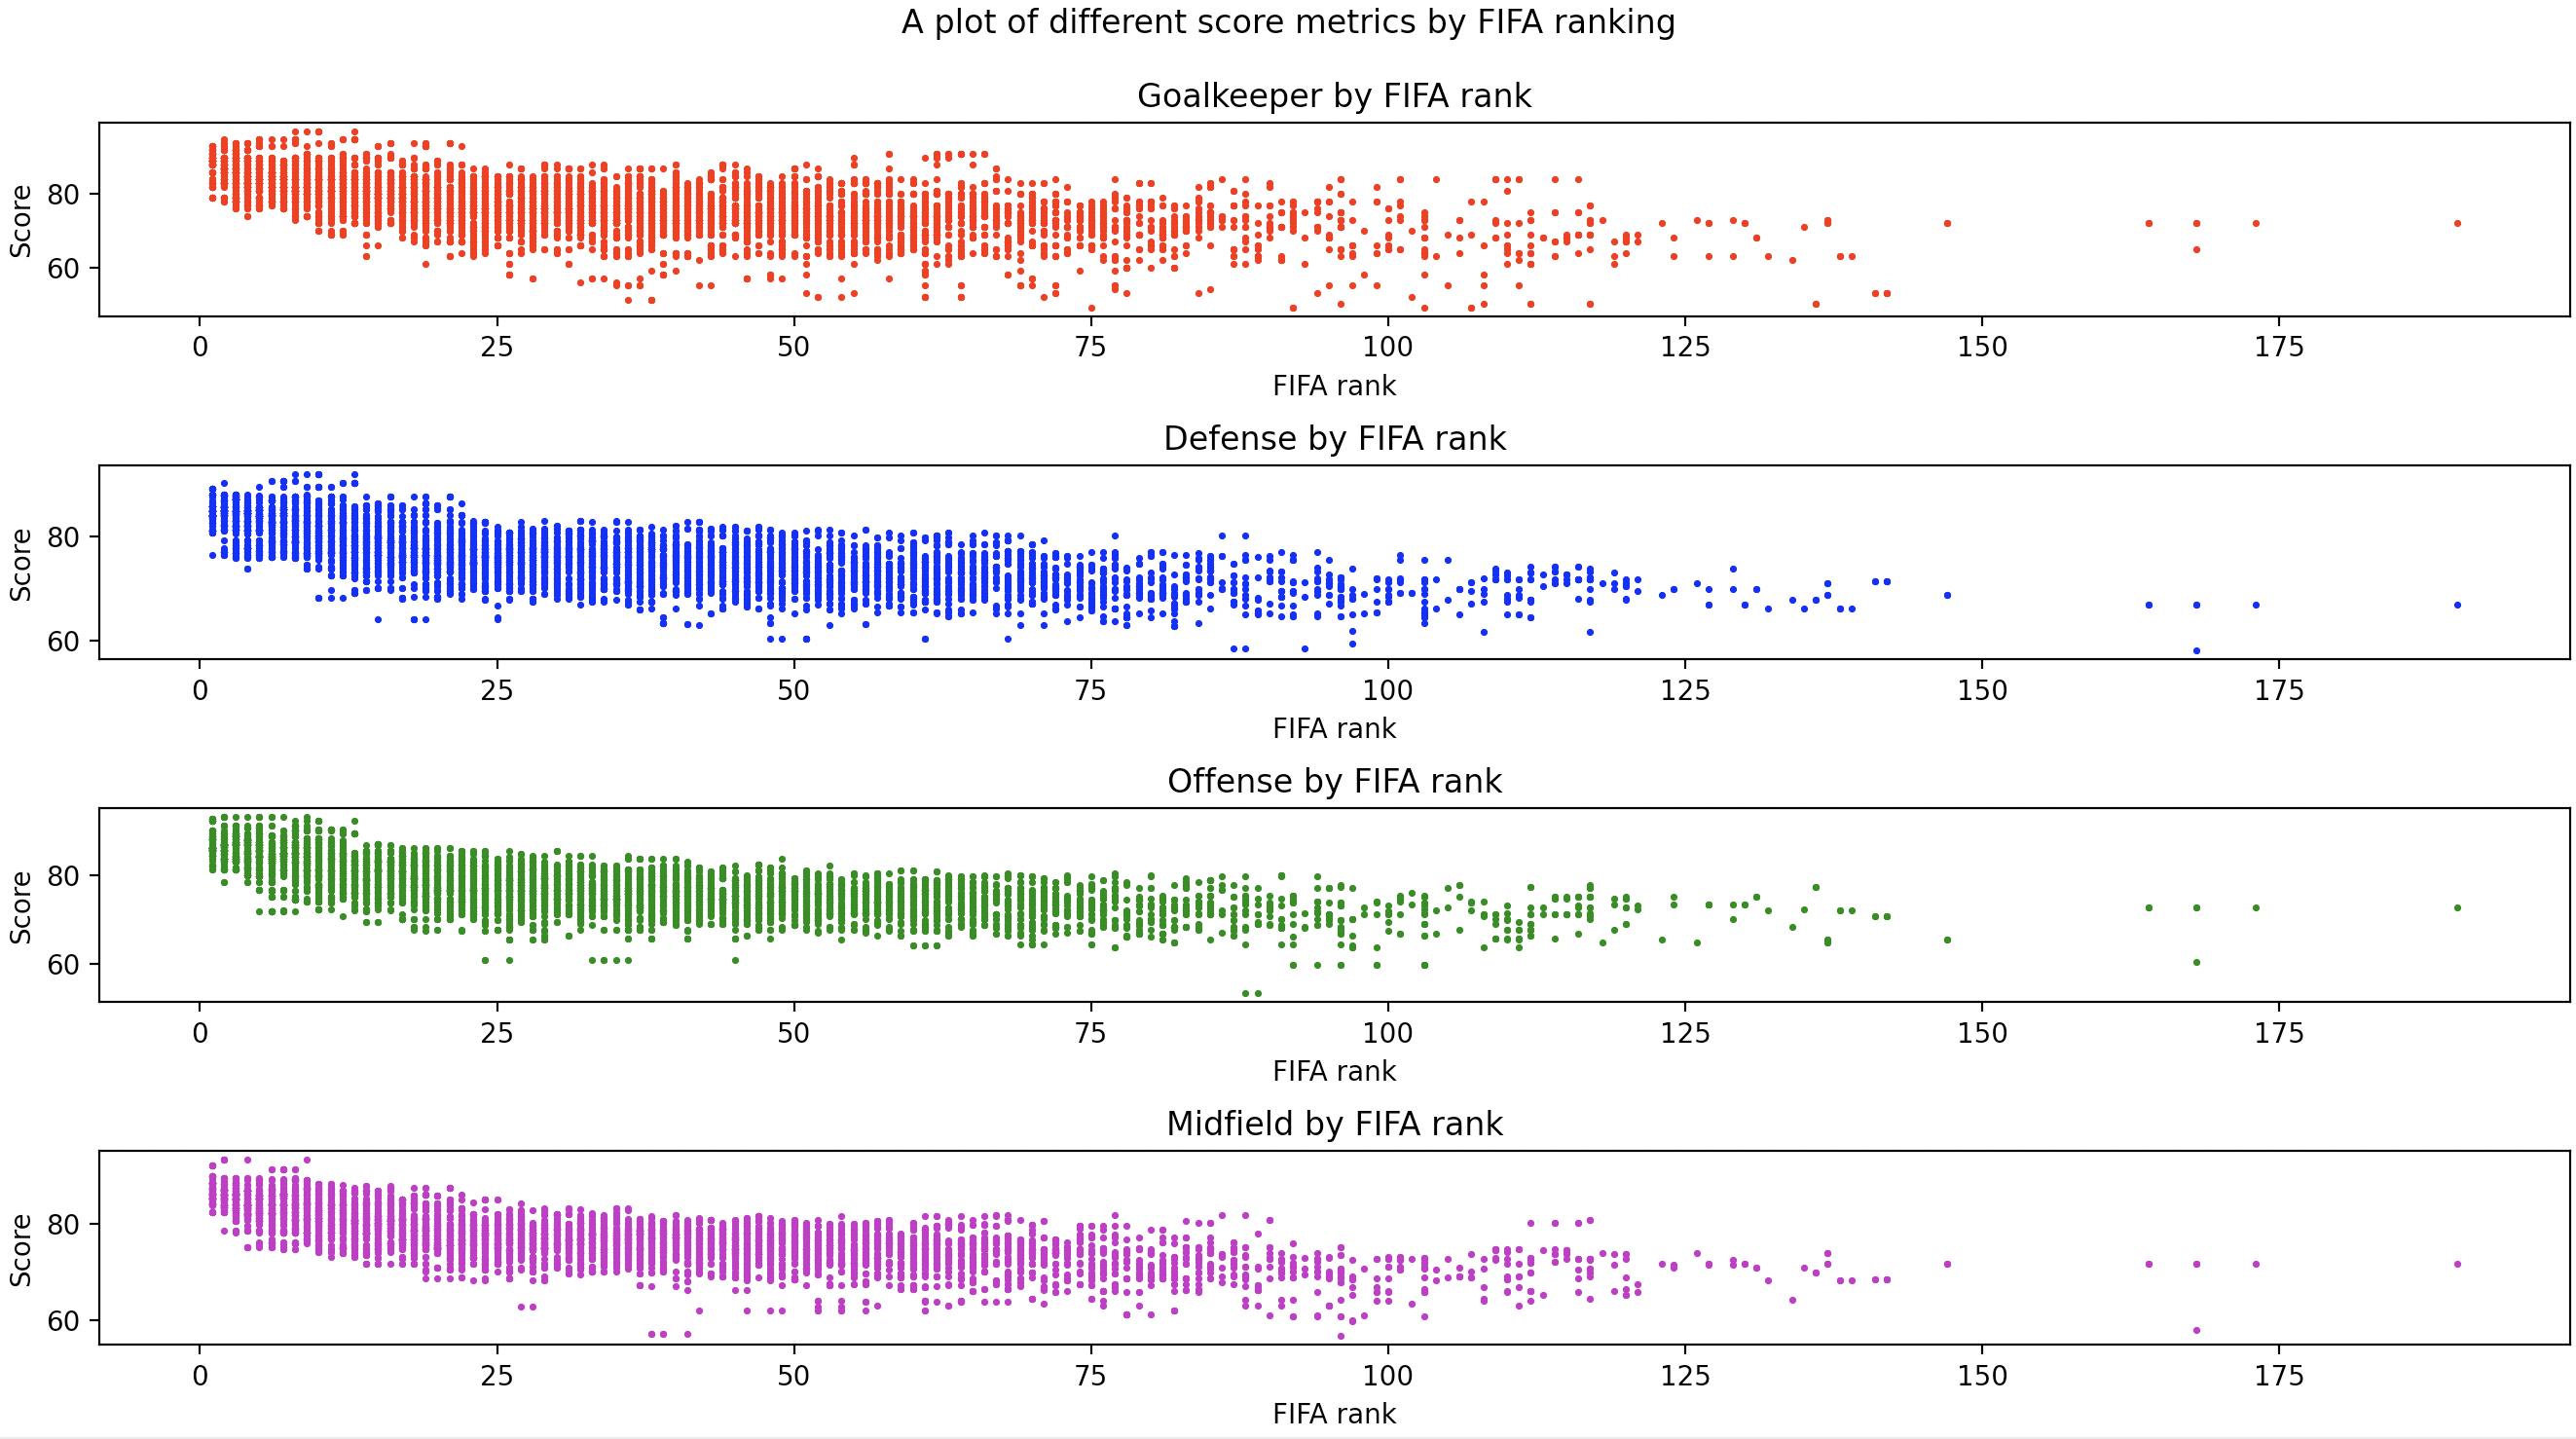
\includegraphics[scale=.3]{scores_plots.png}
    \caption{\textit{goalkeeper\_score, defense\_score, offense\_score, midfield\_score} plotted by country against said country's FIFA ranking.}
    \label{fig:scoreplots}
\end{figure}
Since the values we were concerned with filling were all position scores, we decided to look at the distribution of these features to get a better understanding of what static value we could reasonably replace them with.

\begin{figure}[H]
    \centering
    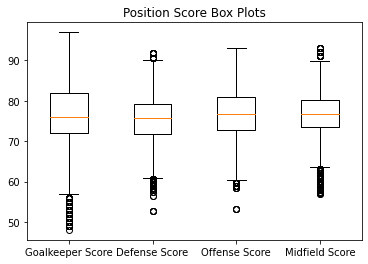
\includegraphics[scale=.6]{box_plots.png}
    \caption{Box plots for \textit{goalkeeper\_score, defense\_score, offense\_score,} and \textit{midfield\_score}.}
    \label{fig:boxplots}
\end{figure}
As shown in the \hyperref[fig:boxplots]{Figure 2}, all of the position features are roughly centred around 75, with tight inter-quartile ranges of about 10. Given that the whiskers didn't extend beyond 15 points above or below the median, this gave us confidence that taking a static value of 75 was reasonable in cases where data was missing. This method was simple and maintained efficiency at run time, while not skewing the data or providing any significant advantage to either team involved.

\subsection{Removal of Rows}
The most naïve approach to dealing with missing data in a dataset is to simply ignore the records that have missing values when training a model. This method is quick and simple to implement. Furthermore, this method's naïvety does not necessarily equate to poor performance. Overall, in the provided dataset of 5642 records, 1525 of them are missing at least one value, meaning that simply removing these rows to generate a new complete dataset, leaves 4117 records to use in model training. We found this to be more than enough to still achieve reasonable model accuracy for each method regression used.

\subsection{Replacing With Dataset Averages}
The next approach we experimented with was to calculate, for each of the features with missing values, the average for the entire dataset and use it to fill in the missing values. 

\subsection{Replacing with Country Averages}
The most involved, and therefore successful method of restoring missing data we found was to replace missing values with the feature average corresponding to the country for which it is missing. For example, in the game between Albania and Greece on the 4th of September 2004, there is no recorded \textit{goalkeeper\_score} for Albania. Therefore, we input Albania's average \textit{goalkeeper\_score} which is calculated using their other international games for which this value is present. Calculating the averages is a simple procedure - looping over the entire dataset while keeping running averages for each missing feature for each country. 

The above method of replacing missing values with averages works well in most circumstances, however, more complexly, there are 151 records which contain a missing value that is missing entirely for one of the countries in the record. For example, in the game between Zambia and Senegal from the 3rd of September 2005, Zambia has no \textit{defense\_score}. It cannot be replaced with Zambia's average \textit{defense\_score} because there are no records for Zambia that contain that feature. 

We tried implementing several different methods for handling these entirely missing features: linear regression using FIFA rank and \textit{pandas.Series.interpolate()}, and a Gaussian distribution.

\subsubsection{Regression With FIFA Rank}
Another attempt to predicting the missing values was to run linear regression on the graphs according to Figure 1. The linear regression model was constructed given the FIFA rank and position score information.

\subsubsection{interpolate()}
\textit{pandas.Series.interpolate()} \cite{interpolate} is a library method than can interpolate values in a dataset in which `NaN' values are present. By creating, for each feature, a \textit{pandas.Series} contaning every instance of that feature (whether it is missing or not) along with the rank of the country for which the value belongs, we can interpolate the missing values. This allows us to, for example, create an artificial value for Zambia's average \textit{defense\_score}. This method of interpolation can be done either linearly or polynomially - looking at the data representation in \ref{fig:score_plots}, linear interpolation was chosen. Below is an example of how the linear interpolation works:

\tiny{
\begin{python}
    >>> s = pd.Series([0, 1, np.nan, 3])
    >>> s
    0    0.0
    1    1.0
    2    NaN
    3    3.0
    dtype: float64
    >>> s.interpolate()
    0    0.0
    1    1.0
    2    2.0
    3    3.0
    dtype: float64
\end{python}
}
\small

\subsubsection{Gaussian Distribution}
Another approach we experimented with was to model a country's position scores as a Gaussian random variable. To do this, we first gathered all records of the country's missing position score from the \textit{match\_history.csv} file. Then, the mean and variance could be calculated using the NumPy functions \textit{mean()} and \textit{var()}. An important decision we made was to use a truncated Gaussian distribution. Extrapolating above or below the observed best and worst performances for a team could potentially bias our data, especially since the Gaussian distribution is symmetrical.
Computationally, this method proved near equivalent to calculating averages. This is because the extra work of calculating the variance and then sampling from the truncated Gaussian distribution was small compared to iterating through the dataset to gather the relevant data.
\begin{figure}[H]
        \centering
        \begin{subfigure}[b]{0.45\textwidth}
            \centering
            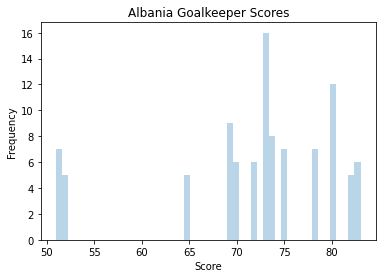
\includegraphics[scale=.4]{albania_scores.png}
            \caption{Real Scores}
        \end{subfigure}
        \hspace{0.5em}%
        \begin{subfigure}[b]{0.45\textwidth}
            \centering
            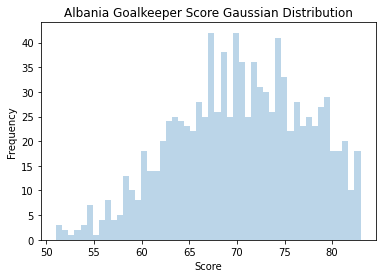
\includegraphics[scale=.4]{albania_gaussian.png}
            \caption{Simulated Scores}
        \end{subfigure}
        \caption{Comparison of real and simulated results for Albania's \textit{goalkeeper\_score}, presented as histograms}
        \label{fig:histograms}
\end{figure}
Using the truncated Gaussian distribution replicated the naturally occurring variance in the data well and without extrapolation. However, this method fell short when dealing with instances of features being completely absent for a country, as mentioned in \hyperref[sec:miss data]{Section 2.2}.

\subsection{Data Exploration}
The objective of the project is to develop a predictive model for the outcomes of football matches. Through a thorough examination of the available data, it was determined that there is a strong correlation between the relative strength of the teams involved and the resulting outcome of the match. Accordingly, this correlation will be taken into account as a key factor in the development of the predictive model. 
Therefore, we mainly focus on the team position score features.

In order to gain a more comprehensive understanding of the position scores, a graph was plotted to illustrate the relationship between the position scores and FIFA rank. This representation allowed for a more lucid analysis of the data, and facilitated a deeper understanding of the underlying trends and patterns.
\begin{figure}[H]
    \centering
    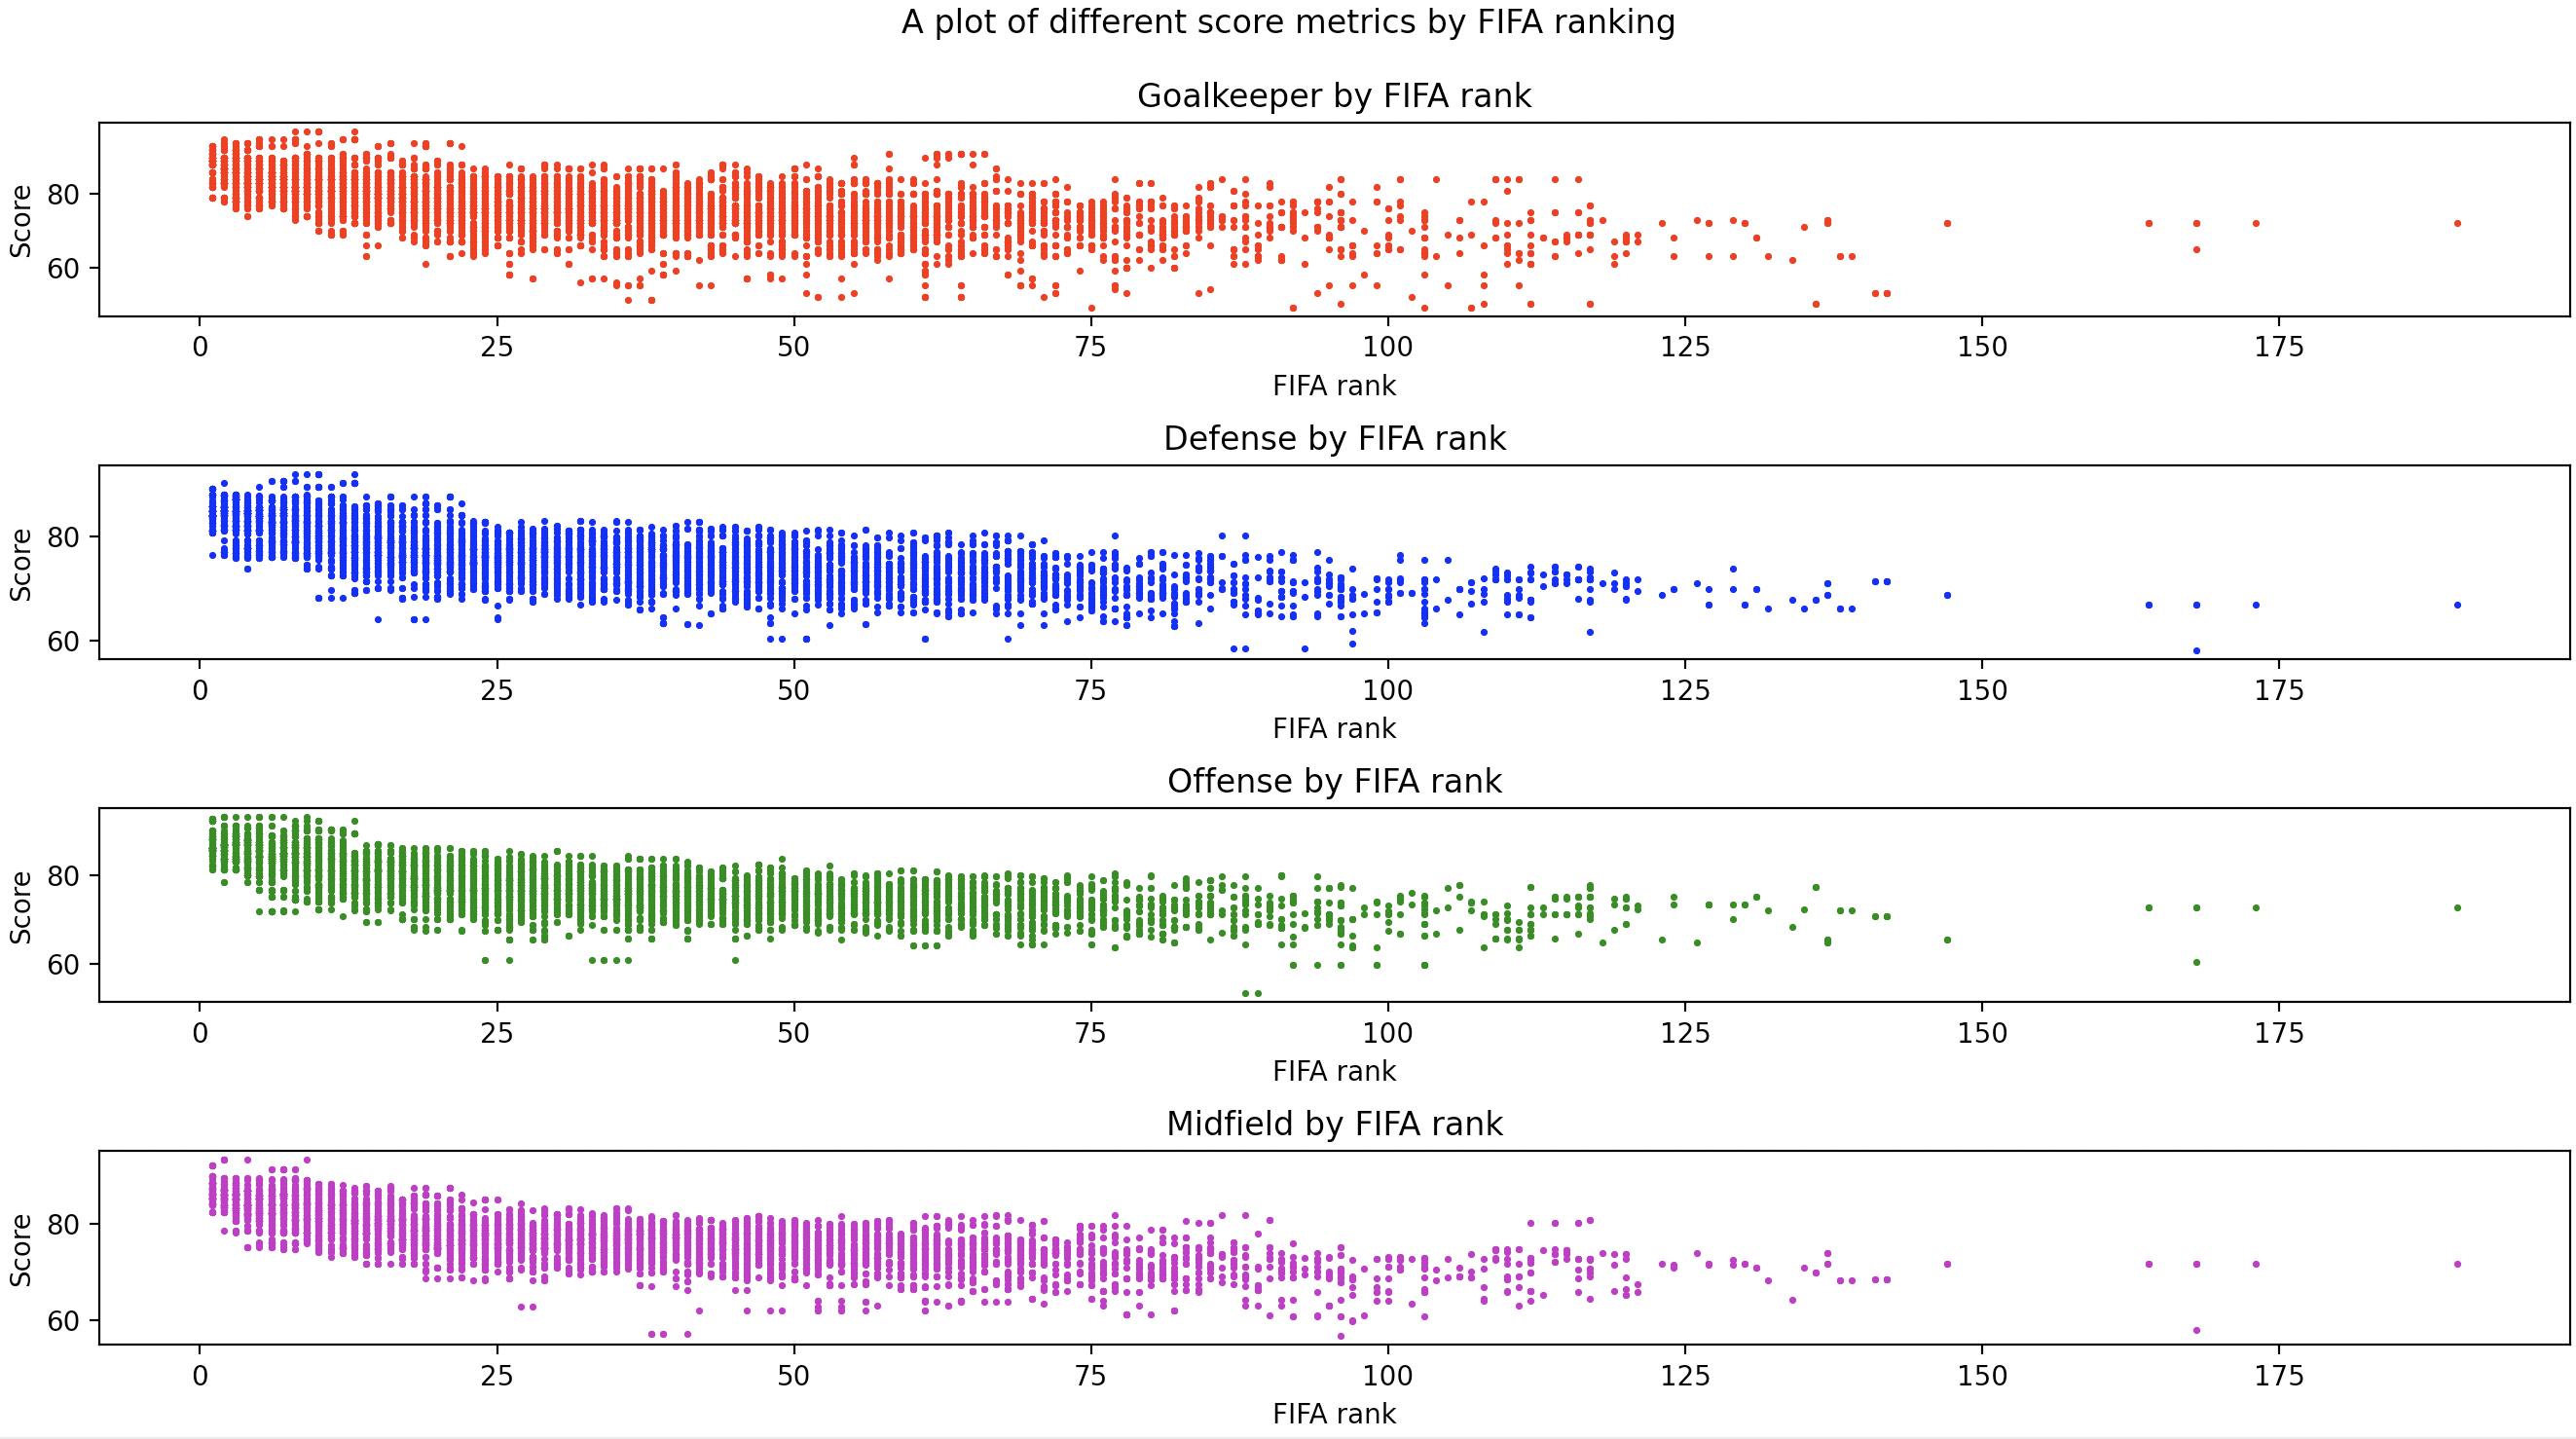
\includegraphics[scale=.3]{scores_plots.png}
    \caption{\textit{goalkeeper\_score, defense\_score, offense\_score, midfield\_score} plotted by country against said country's FIFA ranking.}
    \label{fig:scoreplots}
\end{figure}